\documentclass[11pt, letterpaper]{article}
\usepackage{graphicx}
\usepackage[export]{adjustbox}
\usepackage{hyperref}
\usepackage{xcolor}
\graphicspath{{images/}}
\usepackage[a4paper, total={6in, 8in}]{geometry}
\usepackage{tabularx}
\usepackage{polski}
\usepackage{float}


\title{\textbf {ShotFlow} \\ \large Końcowa specyfikacja}

\author{Michał Kiedrzyński}

\date{Styczeń 2025}


\begin{document}
\maketitle

\newpage
\tableofcontents
\newpage

\section{Opis projektu}
ShotFlow to aplikacja przeznaczona dla zespołów realizacji wizualnej, na wydarzeniach takich jak koncerty, konferencje, czy programy telewizyjne, w których lista kolejnych ujęć może być zaplanowana z wyprzedzeniem. Aplikacja pozwala między innymi na:
\begin{itemize}
    \item śledzenie postępu realizacji w czasie rzeczywstym,
    \item dostarczenie każdemu operatorowi informacji o jego ujęciach,
    \item wyświetlanie informacji czy jest się na wizji niezależnie od aktualnego ekranu,
    \item szybką zmianę planu realizacji w przypadku zmiany sytuacji,
    \item bezpośrednią komunikację z realizatorem poprzez czat,
    \item personalizację wyglądu aplikacji.
\end{itemize}

\subsection{Ekrany}
Aplikacja składa się z kilku ekranów, po których nawigacja jest bardzo intuicyjna.
\subsubsection{Ekran logowania}
\begin{figure}[H]
    \centering
    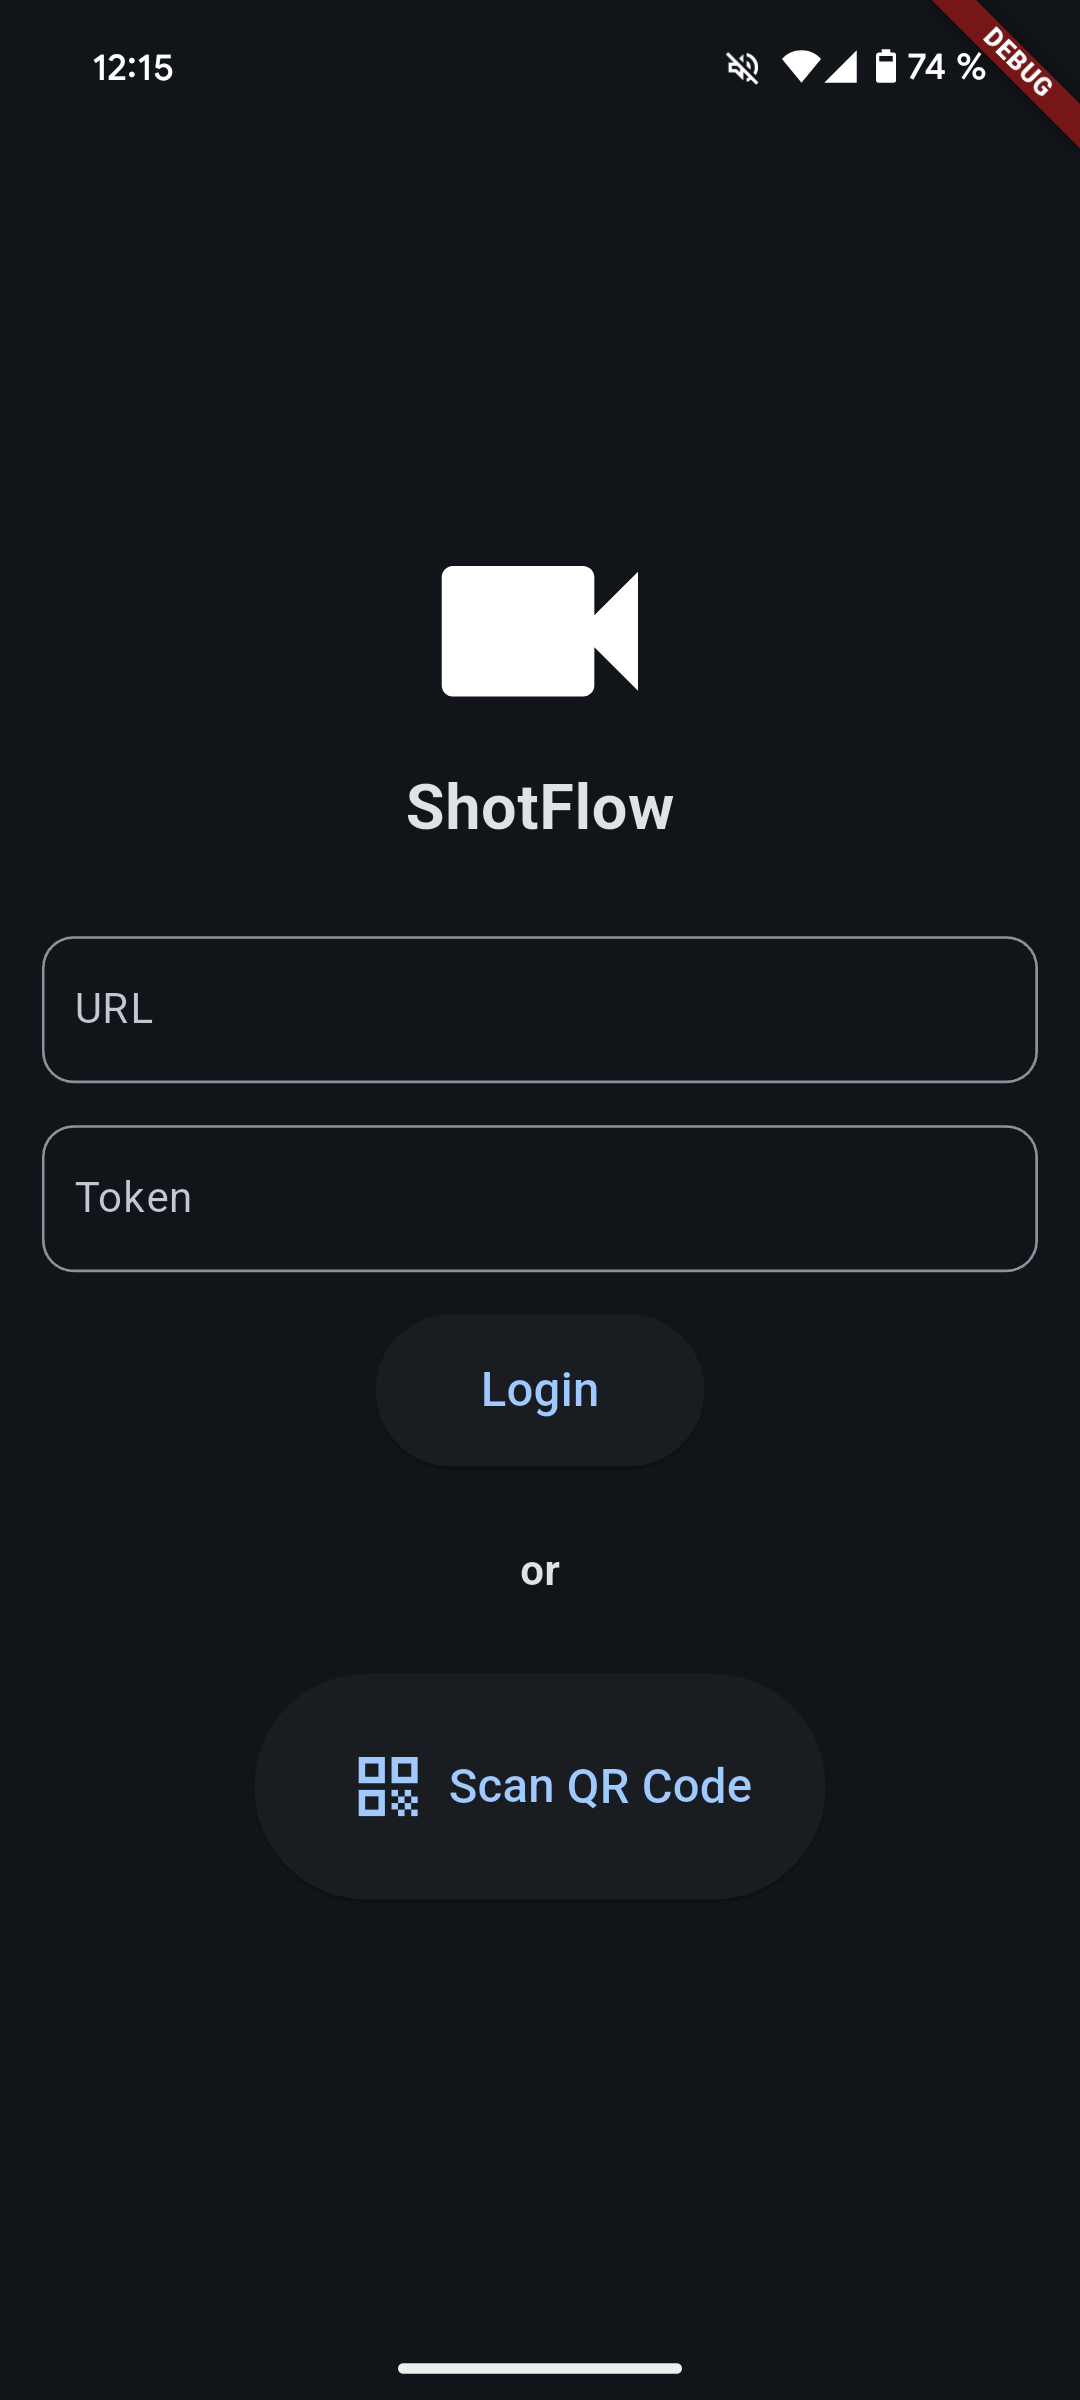
\includegraphics[width=0.3\textwidth]{login.png}
\end{figure}
Na ekranie logowania należy wpisać adres WebSocket serwera (zaczynający się od \texttt{ws://} lub \texttt{wss://}) oraz token autoryzacyjny. Po kliknięciu przycisku \textit{Zaloguj} aplikacja spróbuje połączyć się z serwerem. W przypadku niepowodzenia wyświetli się odpowiedni komunikat.

Dla usprawnienia procesu, możliwe jest również zalogowanie przy pomocy kodu QR, na którym zakodowany jest adres serwera oraz token w formacie JSON:
\begin{verbatim}
    {"url": "ws://example.com","token": "abc"}
\end{verbatim}
Kliknięcie w przycisk \textit{Zeskanuj kod QR} otworzy kamerę, która po zeskanowaniu kodu automatycznie wypełni pola adresu serwera i tokenu, a następnie spróbuje połączyć się z serwerem.

\subsubsection{Ekran ujęć}
\begin{figure}[H]
    \centering
    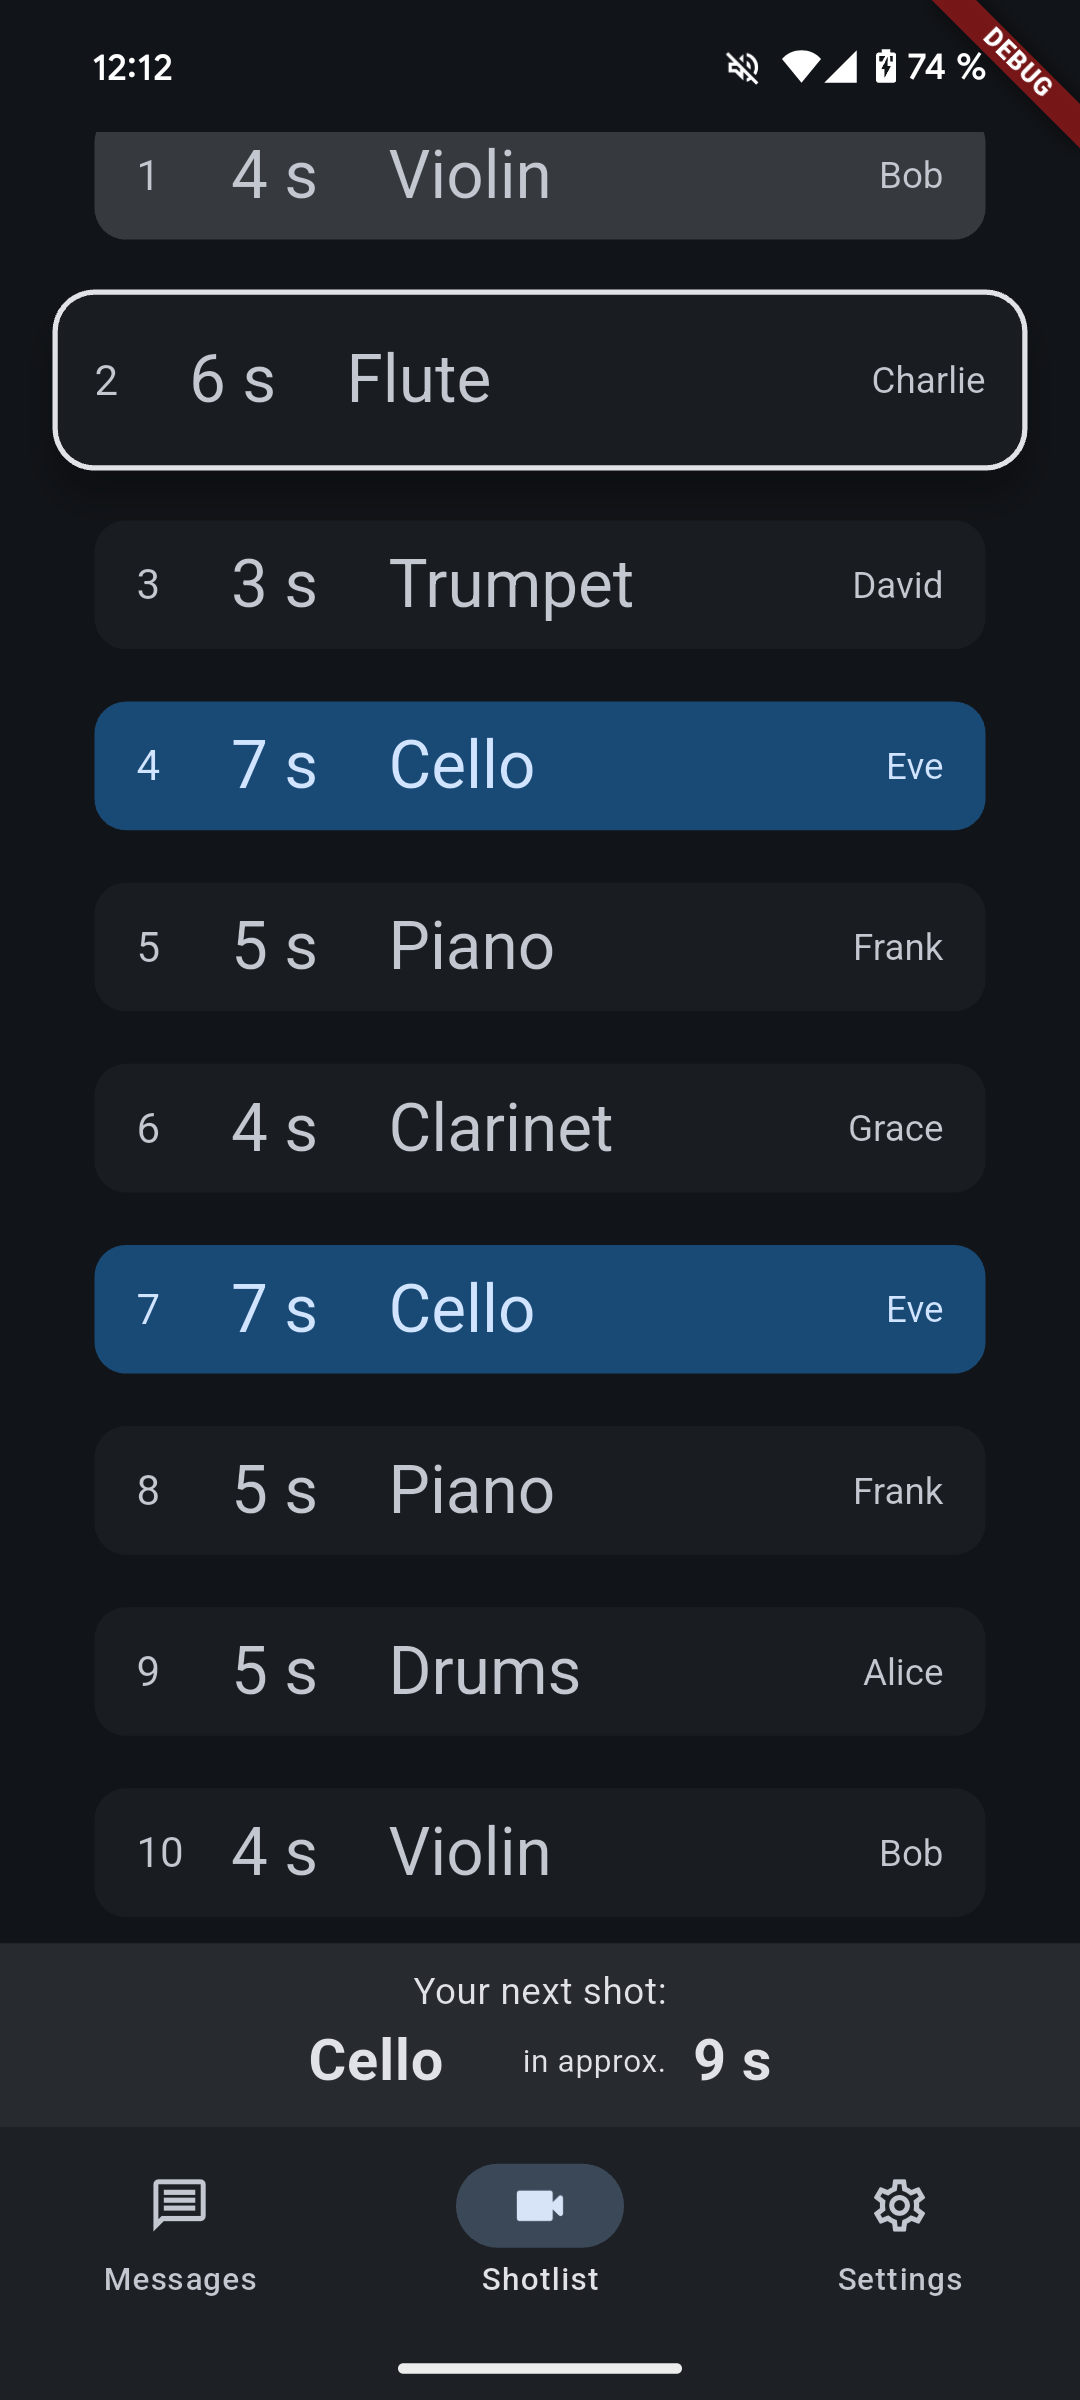
\includegraphics[width=0.3\textwidth]{shotlist.png}
\end{figure}
Po zalogowaniu następuje przekierowanie na główny ekran, jakim jest lista ujęć. Wyświetany jest tutaj aktualny stan transmisji, a sama lista przewija się automatycznie w miarę jej postępu. Ujęcia operatora wyróżnione są kolorem (konfigurowalnym w ustawieniach). Na dole ekranu wyświetlany jest pasek z informacją o kolejnym ujęciu i przybliżonym czasie do jego rozpoczęcia.

Użytkownik może również samodzielnie przewinąć listę, aby zobaczyć inne ujęcia. Automatycznie przewijanie jest wtedy wstrzymywane i w prawym dolnym rogu pojawia się przycisk pozwalający na jego wznowienie.

Dodatkowo, niezależnie od aktualnego ekranu, na całą aplikację nakładana jest ramka, która zmienia kolor na zielony, gdy operator jest następny do wejścia, oraz czerwony, gdy jest na wizji.

\subsubsection{Ekran wiadomości}
\begin{figure}[H]
    \centering
    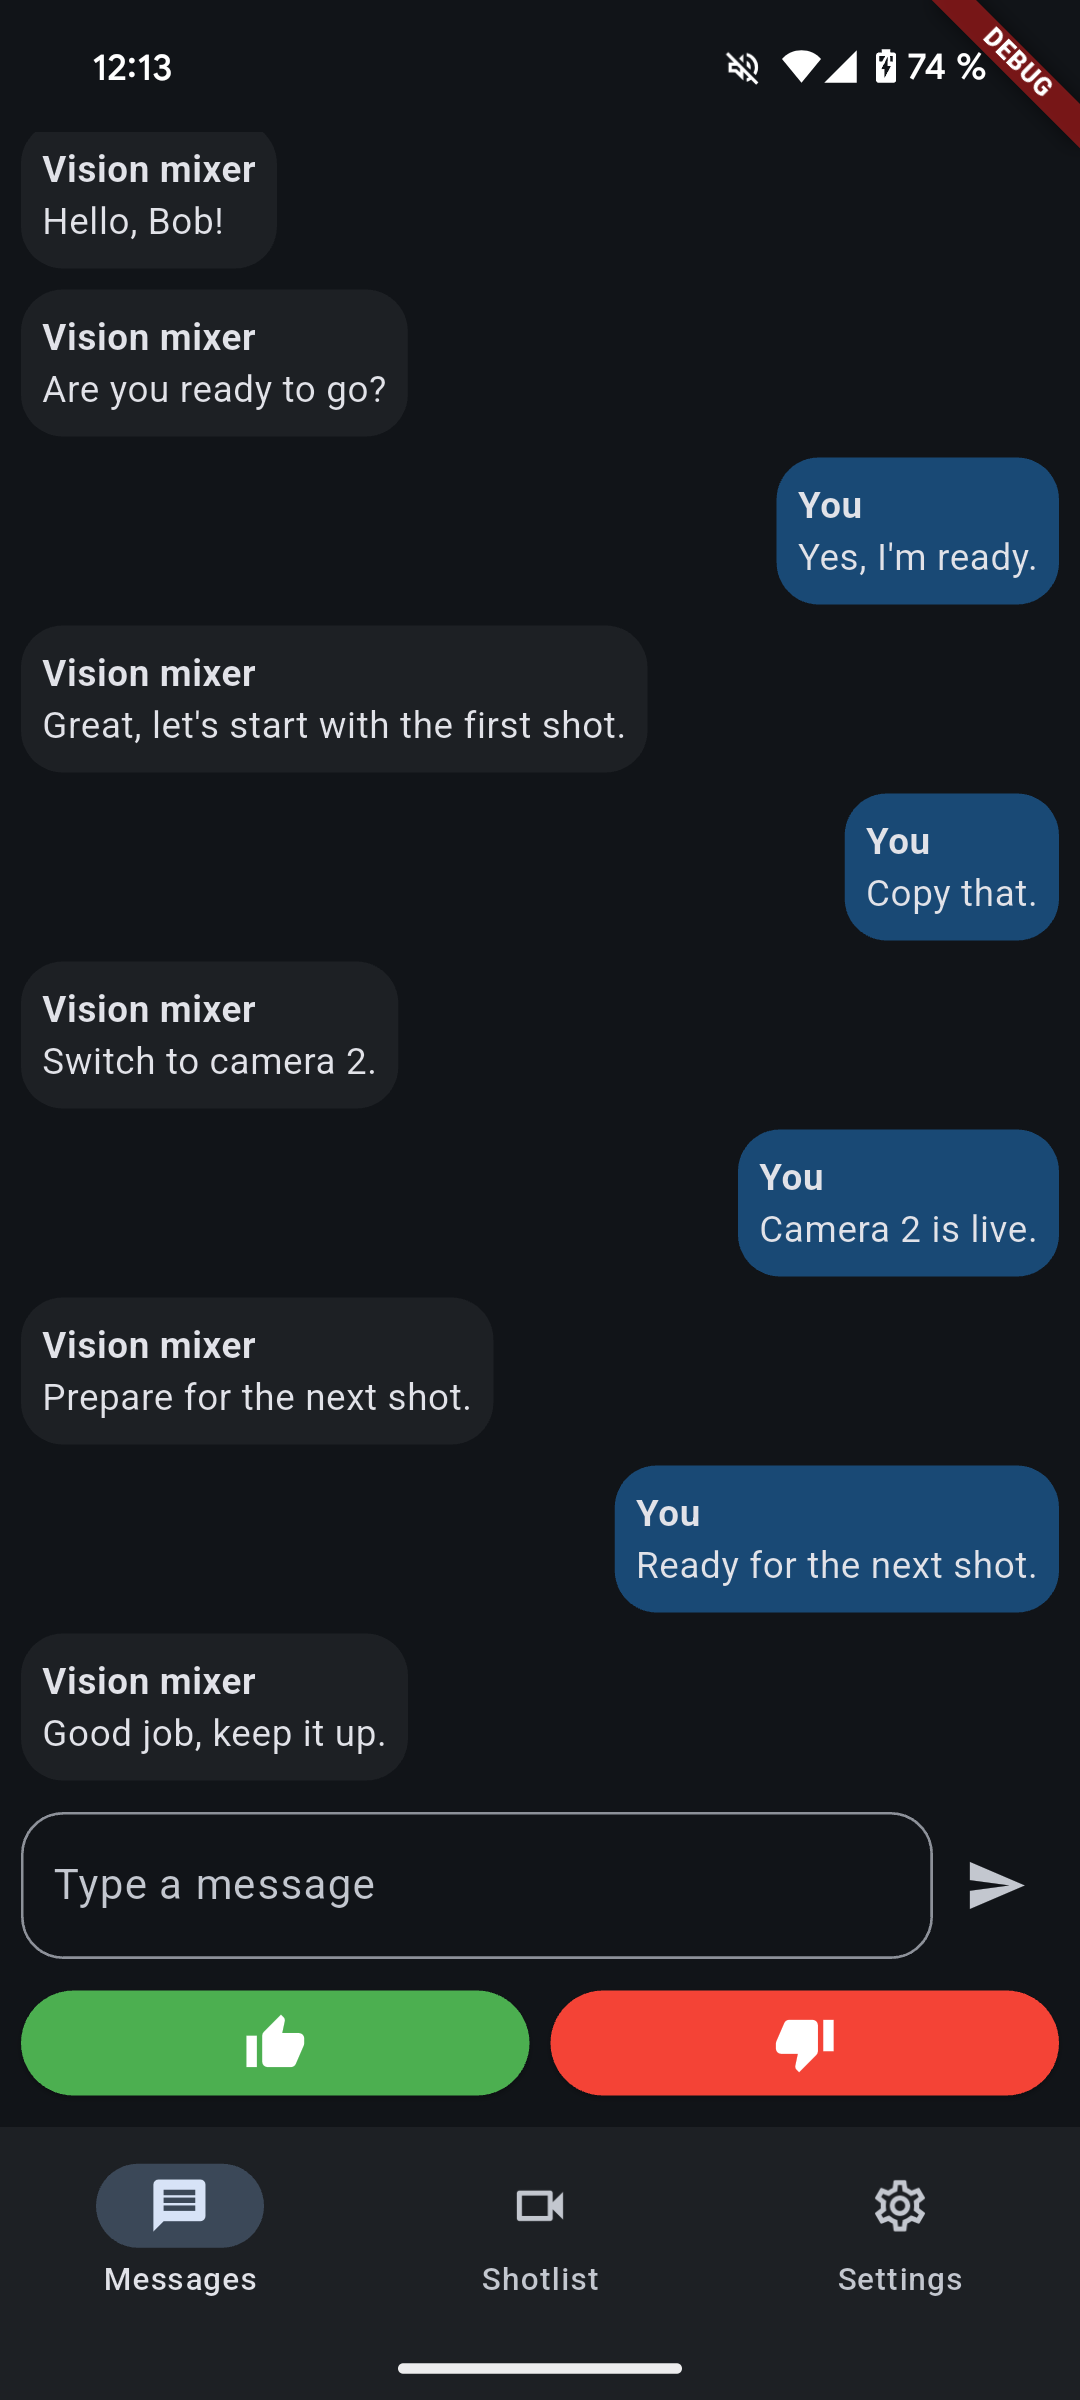
\includegraphics[width=0.3\textwidth]{messages.png}
\end{figure}
Ekran wiadomości pozwala na szybką komunikację z realizatorem w czasie rzeczywistym. Poza standardową metodą wpisywania tekstu, dostępne są również dwa przyciski szybkiej odpowiedzi, aby maksymalnie zaoszczędzić cenny czas w trakcie realizacji.

\subsubsection{Ekran ustawień}
\begin{figure}[H]
    \centering
    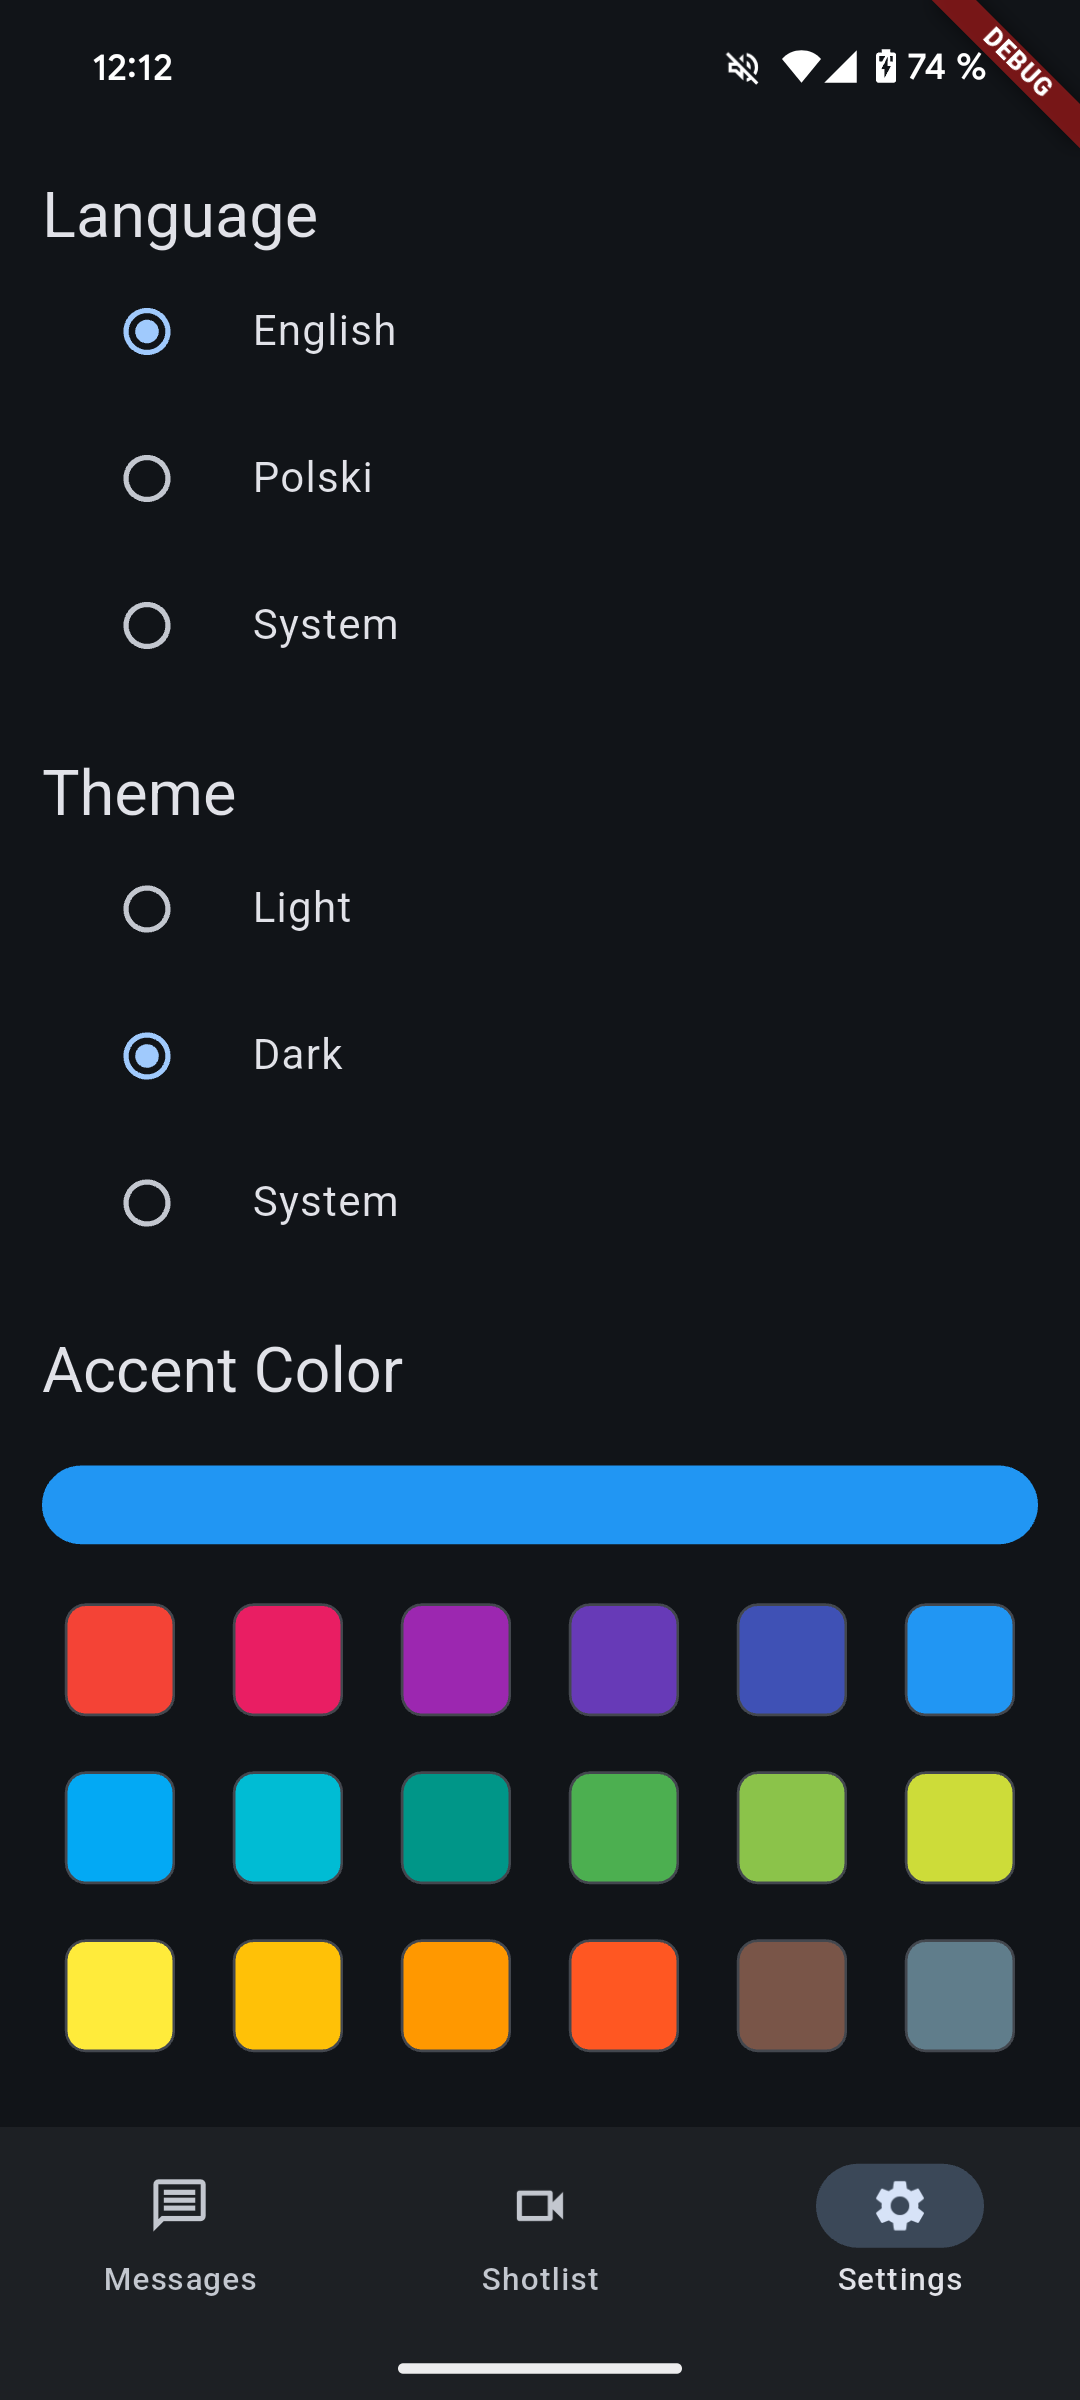
\includegraphics[width=0.3\textwidth]{settings.png}
\end{figure}
Ekran ustawień pozwala na zmianę języka aplikacji, dostosowanie jej wyglądu do własnych potrzeb i preferencji, a także wylogowanie (po przewinięciu w dół).

\subsection{Komunikacja}
System używa własnego serwera, w zamyśle uruchomionego na stacji realizatorskiej. Aplikacja komunikuje się z serwerem przy pomocy protokołu WebSocket. Szyfrowanie komunikacji jest możliwe (protokół WSS), ale nie jest wymagane.
\subsubsection{Logowanie}
Podczas logowania aplikacja ustanawia połączenie z serwerem, a następnie przesyła token autoryzacyjny. W przypadku niepowodzenia serwer zwraca błąd i zrywa połącznie, a aplikacja wyświetla komunikat o nieudanej próbie logowania. W przypadku powodzenia serwer zwraca informację o zalogowaniu, a aplikacja przechodzi do ekranu ujęć.

\subsubsection{Przesłanie listy ujęć}
Aby uniknąć problemów z synchronizacją, aplikacja nie przechowuje listy ujęć lokalnie dłużej niż czas jej życia. Dlatego po każdorazowym zalogowaniu serwer wysyła listę ujęć w formacie:
\begin{verbatim}
{
    "type": "shotlist_update",
    "data": [
        {
        "id": 0,
        "title": "Drums",
        "operator_id": 1,
        "operator_name": "Alice",
        "duration": 5
        },
        {
        "id": 1,
        "title": "Violin",
        "operator_id": 2,
        "operator_name": "Bob",
        "duration": 4
        },
        [...]
    ]
}
\end{verbatim}
Taka wiadomość może zostać wysłana również w trakcie realizacji, jeśli lista ujęć zostanie zmieniona.

\subsubsection{Przypisanie operatora}
Po wysłaniu listy ujęć, serwer nadaje użytkownikom ich identyfikatory, używane do przypisania operatorów do konkretnych ujęć. Dzieje się to poprzez wysłanie wiadomości:
\begin{verbatim}
    {"type": "operator_assign", "operator_id": 5}
\end{verbatim}
Tak jak poprzednio, możliwa jest zmiana id operatora w trakcie realizacji.

\subsubsection{Przesłanie historii wiadomości}
Ze względu na styl komunikacji podczas realizacji (krótkie, szybko przedawniajace się wiadomości) oraz pracę z różnymi realizatorami podczas różnych wydarzeń, aplikacja nie przechowuje historii wiadomości lokalnie. Po zalogowaniu serwer ma jednak możliwość przesłania ostatnich wiadomości, aby zapewnić spójność komunikacji w obrębie jednego wydarzenia. Robi to wysyłając wiadomość:
\begin{verbatim}
{
    "type": "message_history",
    "messages": [
        {"sender": "Vision mixer", "message": "Hello, Bob!"},
        {"sender": "Vision mixer", "message": "Are you ready to go?"},
        {"sender": "You", "message": "Yes, I'm ready."},
        [...]
    ]
}
\end{verbatim}


\subsubsection{Zmiana ujęcia}
W momencie rozpoczęcia kolejnego ujęcia serwer wysyła wiadomość:
\begin{verbatim}
    {"type": "shotlist_jump", "currently_live": 5}
\end{verbatim}
gdzie \texttt{currently\_live} to id ujęcia, które właśnie się rozpoczyna.


\section{Zaimplementowane dodatkowe wymagania}
\begin{itemize}
    \item Aplikacja działa na systemach Android oraz Windows, a także w wersji webowej.
    \item Ikonki na głównym pasku nawigacyjnym mają customowe animacje.
    \item Aplikacja posiada testy jednostkowe.
    \item Logowanie następuje przy pomocy własnej metody autoryzacji z serwerem.
    \item Na platformach Android oraz Web dostępna jest możliwość logowania przy pomocy kodu QR przy użyciu kamery.
    \item Aplikacja działa w językach polskim i angielskim.
    \item Aplikacja przechowuje lokalnie ustawienia użytkownika (język, kolorystyka) przy użyciu \textit{shared\_preferences} oraz url serwera i token autoryzacyjny w bezpieczny sposób, przy użyciu \textit{flutter\_secure\_storage}.
\end{itemize}

\section{Przykładowy serwer}
Do aplikacji dołączony jest przykładowy serwer w C\#. Serwer ten jest bardzo prosty i służy jedynie do demonstracji działania aplikacji. Wykonuje on sekwencję logowania, a następnie co 3 sekundy przewija listę ujęć. Na wiadomości wysłane przez czat odpowiada echem.

Dla poprawnego działania serwera może być konieczne manualne otworzenie portu w zaporze sieciowej systemu.

\end{document}